\documentclass{article}
\usepackage{enumitem,amssymb}
\usepackage{tcolorbox}

\usepackage[T1]{fontenc}
\usepackage[utf8]{inputenc}
\usepackage{tgbonum}
\usepackage[normalem]{ulem}
\usepackage{float} %to place figures where they are in the source with [H]

\newcommand*{\TakeFourierOrnament}[1]{{%
\fontencoding{U}\fontfamily{futs}\selectfont\char#1}}
\newcommand*{\danger}{\TakeFourierOrnament{66}}
\color{black}

\usepackage[includehead,includefoot]{geometry}
 \geometry{
 a4paper,
 left=10mm,
 top=20mm,
 right=80mm,
 bottom=20mm
 }

\usepackage{fancyhdr}
\fancyhf{µHoubolt EuRoC Launch Procedures}
\fancyfoot[R]{}
\rhead{v2.3}
\pagestyle{fancy}
%\lhead{\LaTeX{} tutorials}
 
\newcommand\checkbox[0]{ \hfill $\msquare$}
\newcommand\leftcheckbox[0]{ \hfill $\msquare$\hphantom{abcd}}
\newcommand\warningcheckbox[0]{ \hfill $\msquare$\danger}
\newcommand\warningleftcheckbox[0]{ \hfill $\msquare$\danger\hphantom{cd}}
\newcommand\twoCheckboxes[0]{ \hfill Ox$\msquare$ Fuel$\msquare$}
\newcommand\twoLeftCheckboxes[0]{ \hfill Ox$\msquare$ Fuel$\msquare$\hphantom{abcd}}
\newcommand\timestampcheckbox[0]{\hfill\dotuline{\hphantom{00:00:}}\hphantom{a}$\msquare$}


\newcommand\underlined[0]{\hphantom{ab}\dotfill\hphantom{abcd}}
\newcommand\underlinedWithBrackets[0]{\hphantom{ab}\dotfill(\hphantom{abcde})\hphantom{abcd}}
\newcommand\shortunderlined[0]{\hphantom{ab}\dotfill\hphantom{a}}
\newcommand\task[1]{\hrulefill\hphantom{ab} #1 \hphantom{ab}\hrulefill}
\newcommand\starttask[2]{\bigskip \hrulefill \break \textbf{#1} \hfill\break \textbf{#2}}
\newcommand\codeblock[1]{{\fontfamily{qcr}\selectfont #1 }}


\usepackage{scalerel,amssymb}
\def\msquare{\mathord{\scalerel*{\Box}{gX}}}

\usepackage{siunitx}
\usepackage{hyperref}
%ToDo List
% finish pressurant checklist
% check everything
% 
%
%



\title{µHoubolt Launch Procedures}
\author{TU Wien Space Team}
\date{February 2021}

\begin{document}
%{\fontfamily{qcr}\selectfont
%{\fontfamily{phv}\selectfont
%{\fontfamily{qag}\selectfont
{\fontfamily{qhv}\selectfont

%\maketitle
%\clearpage
\newpage
\setcounter{page}{1}
\lhead{Lead}
\lfoot{\thepage / \pageref{end_section_lead}}
\section*{Lead}
\begin{tcolorbox}
\color{black}

\textbf{Important Note:}\\
Tasks for Mission Control are \underline{underlined}. Mission Control needs to be told every underlined instruction.\\
Ensuring that tasks on your checklist are done is \textbf{your} responsibility.\\
Always request acknowledgement from Mission Control and verify yourself if possible.
\end{tcolorbox}
\begin{tcolorbox}
\color{black}

\textbf{Legend:}\\
CAN \underlined Controller Area Network; Data bus (orange cable)\\
ECU \underlined Engine Control Unit\\
ECUI \underlined Engine Control User Interface\\
GSE \underlined Ground Support Equipment\\
iperf \underlined Network testing tool\\
LCO \underlined Launch Control Officer\\
LRR \underlined Launch Readiness Review\\
MC \underlined Mission Control\\
PMU \underlined Power Management Unit\\
PoE \underlined Power over Ethernet\\
%PTFE seal \underlined Teflon sealing tape\\
RBF \underlined Remove Before Flight\\
RCU \underlined Radio Control Unit\\
TRS \underlined Total Recovery System (Eggtimer)\\
T<number> \underlined Torx driver of specified size\\\\

Requests \underlined Always wait for acknowledgement\\
Instruct \underlined Acknowledgment comes later\\
Check \underlined Only assessment, no corrective actions\\
Verify \underlined Corrective action included
\end{tcolorbox}

\begin{enumerate}[label=L\arabic*.]
    \item READ THE WHOLE CHECKLIST BEFORE STARTING \checkbox
    
    \starttask{Required tools, materials and personnel}{\hphantom{a}}
    \item \label{lead_personnel} Personnel
        \begin{enumerate}[label*=\arabic*.]
            \item Mission Lead: Georg Mikula
        \end{enumerate}
    \item \label{lead_tools} Tools
        \begin{enumerate}[label*=\arabic*.]
            \item Pen\checkbox
        \end{enumerate}
    
    \starttask{Pre-Launch Prep}{\hphantom{a}}
    \item Instruct Pad Prep personnel to start with Pad Prep checklist. (\ref{pad_prep_start}-\ref{pad_prep_end})\checkbox
    \item Instruct Rocket prep personnel to start non-energetic rocket assembly (\ref{rocket_non_energetic_start}-\ref{rocket_non_energetic_end}).\checkbox
    
    \starttask{Launch Day}{\hphantom{a}}
    \item Request igniter preparation(\ref{rocket_prep_igniters_start}-\ref{rocket_prep_igniters_end}).\checkbox
    \item Instruct Pad prep personnel to start with Pad prep checklist (\ref{pad_prep_start}-\ref{pad_prep_end}) if not already done, otherwise instruct Pad personnel to start On-Day pad prep checklist (\ref{pad_on_day_elec_start}-\ref{pad_on_day_elec_end}).\checkbox
    \item Request Mission Control Area Clearance from EuRoC staff, if clearance is given, instruct MC preps (\ref{mc_prep_start}-\ref{mc_prep_end}).\checkbox
    
    
    \item Wait for non-energetic rocket assembly completion (\ref{rocket_non_energetic_end}.\checkbox
    \item Request energetics rocket assembly clearance from EuRoC staff.\checkbox
    \item Instruct energetics rocket assembly (\ref{rocket_energetic_start}-\ref{rocket_energetic_end}).\checkbox
    \item Wait for pad prep completion (\ref{pad_prep_end}).\checkbox
    \item Wait for energetics rocket assembly(\ref{rocket_energetic_end}).\checkbox
    \item Request LRR.\checkbox
    \item PASS LRR.\checkbox
    \item If MC clearance wasn't given before, request clearance from EuRoC staff and if given, instruct MC preps (\ref{mc_prep_start}-\ref{mc_prep_end}).\checkbox
    \item Wait for On-Day electronics check to be completed (\ref{pad_on_day_elec_end}).\checkbox
    \item Request clearance for final rocket assembly from EuRoC staff.\checkbox
    \item Request final rocket assembly (\ref{rocket_final_start}-\ref{rocket_final_end}).\checkbox
    \item Request rocket mounting from Pad personnel (\ref{pad_rocket_mounting_start}-\ref{pad_rocket_mounting_end}).\checkbox
    \item Request Fueling from pad personnel (\ref{pad_fueling_start}-\ref{pad_fueling_end}).\checkbox
    \textcolor{gray}{\begin{itemize}
        \item  Wait for fueling request from Lead.\leftcheckbox
        \item Verify fuel main valve is closed.\leftcheckbox
        \item Fill fueling syringe with \SI{950}{\milli\liter} ethanol\leftcheckbox
        \item Fuel \SI{900}{\milli\liter} \leftcheckbox
        \item Clean up spills\leftcheckbox
        \item Mount fincan to rocket\leftcheckbox
        \item Secure fincan with 8 screws\leftcheckbox
        \item Remove cover from oxidizer loading port\leftcheckbox
        \item Connect Ox umbilical\leftcheckbox
        \item Verify Ox umbilical mechanical connection (pull umbilical), reconnect if loose\leftcheckbox
        \item Report that fueling is completed to Mission Lead.\leftcheckbox
    \end{itemize}}
    
    \item \underline{Clear Flash}\checkbox
    \newpage
    \starttask{Oxidizer Filling}{\hphantom{a}}
    \item Verify ox tanking closed\checkbox    
    \item Verify ox vent open\checkbox    
    \item Verify pressurant tanking closed\checkbox    
    \item Verify pressurant vent open\checkbox
    \item Cycle Holddown servo (open, then close)\checkbox
    \item Preliminary internal Go/NoGo Poll\checkbox
        \begin{enumerate}[label*=\arabic*.]
            \item Pad \leftcheckbox
            \item Mission Control \leftcheckbox
        \end{enumerate}
    \item Wait for Launch Window imminent (\SI{30}{\minute})\checkbox
    \item Internal Go/NoGo Poll\checkbox
        \begin{enumerate}[label*=\arabic*.]
            \item Pad \leftcheckbox
            \item Mission Control \leftcheckbox
        \end{enumerate}
    \item Request Final Preps from pad personnel (\ref{pad_final_preps_start}-\ref{vacate_pad}).\checkbox
    \textcolor{gray}{\begin{itemize}
        \item Wait for Mission Lead to request Final Preps\leftcheckbox
        \item Unfold emergency umbilical release line and extend line away from pad \leftcheckbox
        \item Clean intake filters for water pumps \leftcheckbox
        \item Put on safety glasses, gloves, hearing protection and long sleeved shirt and trousers.\leftcheckbox
        \item Verify holddown closed\leftcheckbox
        \item Start pad cams\leftcheckbox
        \item Request Pressurization clearance from EuRoC LCO\leftcheckbox
        \item Raise red pendant\leftcheckbox
        \item Open Ox bottle\leftcheckbox
        \item Open Pressurant bottle\leftcheckbox
        \item Read out pressurant bottle pressure and forward to\newline Mission Lead.\leftcheckbox
        \item Start flight on TRS\leftcheckbox
        \item Remove RBF zip tie \leftcheckbox
        \item Remove RBF umbilical locking device \leftcheckbox
        \item Pull RBF pin\leftcheckbox
        \item Report Final preps complete to Mission Lead.\leftcheckbox
        \item Vacate pad\leftcheckbox
    \end{itemize}}
    
%    \item Check igniters deactivated\checkbox    
%    \item Install igniters \checkbox 
%    \begin{itemize}
%        \item Use fresh PTFE seal\leftcheckbox
%        \item E-match side up\leftcheckbox
%        \item Note which igniter (0/1/2/…) installed where (A/B)\leftcheckbox
%        \item Fully tighten screws\leftcheckbox
%        \item Cable manage igniters with cable tie or aluminium tape\leftcheckbox
%    \end{itemize}

    \item \underline{Verify igniter continuity. Igniter indicators should be yellow in ECUI} \checkbox
    
    \item Verify ox main closed\checkbox    
    \item Set Supercharge 30bar, Hysteresis 1bar\checkbox    
    \item Enable Supercharge pressure control\checkbox    
    \item Close pressurant vent\checkbox
    
    \item Pre-Pressurize tanks\checkbox
     \begin{enumerate}[label*=\arabic*.]
            \item Open pressurant tanking \leftcheckbox
            \item After supercharge opens, close pressurant tanking immediately \leftcheckbox
      \end{enumerate}
    \item Close ox vent\checkbox
    \item Open ox tanking over a duration of \SI{10}{\second}\checkbox
    \item Activate heating cycle\checkbox
    \item After first plume, close ox tanking immediately\checkbox
    \item Activate cooling cycle\checkbox
    \item \label{ox_top_off} Top off Oxidizer
        \begin{enumerate}[label*=\arabic*.]
            \item Wait for stable vent frequency \leftcheckbox
            \item Open ox tanking over a duration of \SI{10}{\second} \leftcheckbox
            \item After first plume, close ox tanking immediately \leftcheckbox
        \end{enumerate}
    \item In case of Hold or Delay of launch window, repeat \ref{ox_top_off} until final GO.
    \item Open Ox vent\checkbox
    
    \item Wait for Launch Window\checkbox
%    \item Enable internal cameras \checkbox
    \item Set Supercharge 60bar, Hysteresis 1bar\checkbox
    \item Open pressurant tanking\checkbox
    \item Wait for stable pressures\checkbox
    \item Close pressurant tanking\checkbox    
    \item Open pressurant vent \checkbox
    
    \starttask{Launch}{\hphantom{a}}
    \item Go/NoGo for launch from EuRoC staff\newline (TRS camera points to receiver)\checkbox
    \item Activate umbilical retract\checkbox
    \item Verify clean separation visually (network camera)\checkbox
    %\item Deactivate charging.\checkbox
    \item Launch\checkbox
    
    \newpage
    \starttask{Safe GSE}{\hphantom{a}}
    \item \label{lead_gse_safing} Request GSE Safing from Pad crew (\ref{pad_gse_safing_start}-\ref{pad_gse_safing_end}).\checkbox
    \item Open ox tanking\checkbox
    \item Open pressurant tanking\checkbox
    \item Verify all pressures are ambient\checkbox
    \item Announce "safe state"\checkbox
    \item Stop network cameras\checkbox
    \item Stop pad cameras\checkbox
 
    \starttask{Safe GSE and Rocket after Abort}{\hphantom{a}}
    Rocket is fully pressurized
    \item Open supercharge\checkbox
    \item Close supercharge after pressure in tank is ambient\checkbox
    \item Open fuel main OR Wait for fuel bleed to vent\checkbox
    \item Go to \ref{lead_gse_safing} \checkbox
    


%    \starttask{Recycle after Abort}{\hphantom{a}}
    
    
%    \item \checkbox
%    \item \checkbox
%    \item \checkbox
%    \item \checkbox
%    \item \checkbox

\label{end_section_lead}
\end{enumerate}
 \cleardoublepage
\newpage
\setcounter{page}{1}
\lhead{Pad Prep}
\lfoot{\thepage / \pageref{end_section_pressurant}}
\section*{Pad Preparation}
\begin{tcolorbox}
\color{black}

\textbf{Legend:}\\
CAN \underlined Controller Area Network; Data bus (orange cable)\\
ECU \underlined Engine Control Unit\\
ECUI \underlined Engine Control User Interface\\
GSE \underlined Ground Support Equipment\\
iperf \underlined Network testing tool\\
LCO \underlined Launch Control Officer\\
LRR \underlined Launch Readiness Review\\
MC \underlined Mission Control\\
PMU \underlined Power Management Unit\\
PoE \underlined Power over Ethernet\\
%PTFE seal \underlined Teflon sealing tape\\
RBF \underlined Remove Before Flight\\
RCU \underlined Radio Control Unit\\
TRS \underlined Total Recovery System (Eggtimer)\\
T<number> \underlined Torx driver of specified size\\\\

Requests \underlined Always wait for acknowledgement\\
Instruct \underlined Acknowledgment comes later\\
Check \underlined Only assessment, no corrective actions\\
Verify \underlined Corrective action included
\end{tcolorbox}

IF A CHECK FAILS AND NO OTHER MEASURE IS SPECIFIED OR THE SPECIFIED MEASURE FAILS TOO, INFORM MISSION LEAD AND AWAIT FURTHER INSTRUCTIONS

\begin{enumerate}[label=PP\arabic*.]

    \item READ THE WHOLE CHECKLIST BEFORE STARTING \checkbox

    \starttask{Required tools, materials and personnel}{\hphantom{a}}
    \item \label{pad_prep_personnel} Personnel
        \begin{enumerate}[label*=\arabic*.]
            \item GSE lead: Johann Breyner
            \item 1 Electronics crew as temporary MC: Markus Pinter
            \item Pad prep crew 1: Florian Dellekart
            \item Pad prep crew 2: Amir Vafaie
            \item Pad prep crew 3: Bernhard Hansemann
        \end{enumerate}
    \item \label{pad_prep_tools} Tools
        \begin{enumerate}[label*=\arabic*.]
            \item Hammer\leftcheckbox
            \item T10 Key\leftcheckbox
            \item T30 Key\leftcheckbox
            \item Allen Key \SI{2.5}{\milli\meter}\leftcheckbox
        \end{enumerate}
    \item \label{pad_prep_materials} Materials
        \begin{enumerate}[label*=\arabic*.]
            \item 1x Launch rail base\leftcheckbox
            \item 2x Launch rail truss\leftcheckbox
            \item 2x \SI{2}{\meter} rail section\leftcheckbox
            \item 1x \SI{1}{\meter} rail section\leftcheckbox
            \item 2x Launch rail struts\leftcheckbox
            \item Propellant loading cart\leftcheckbox
            \item Server rack\leftcheckbox
            \item Flame deflector + safety wires
            \item 3x Guy Cable (ratchet strap + rope + carabiner)\leftcheckbox
            \item 6x Truss connection pins + cross pins\leftcheckbox
            \item 3x Tent pegs\leftcheckbox
            \item 6x Sliding blocks\leftcheckbox
            \item 6x Rail mounting screws\leftcheckbox
            \item \SI{50}{\liter} water in water tanks.\leftcheckbox
            \item \SI{10}{\liter} Water for pad crew. (Canisters \& small bottles)\leftcheckbox
            \item Blue trailer tarp\leftcheckbox
            \item Garbage Bag\leftcheckbox
        \end{enumerate} 
    
    \starttask{Pad preparation}{\hphantom{a}}
    
    \item \label{pad_prep_start} Place trailer towards the left side of the launch pad (apply breaks, extend legs, extend trolley wheel)\checkbox
    \item Remove all equipment except launch rail and tanking cart from trailer \checkbox
    \item Check if all equipment listed in section \ref{pad_prep_materials} is present and in working order \checkbox
    \item Shift oxidiser loading cart to correct position \checkbox
    \item Assemble launch rail in horizontal position \checkbox
    \item Install guy cables on launch rail truss \checkbox
    \item \label{rail_angle} Raise rail to launch angle \newline(84°+-1° pitch, 0°+-1° roll, see bubble levels) \checkbox
    \item Tension and secure guy cables \checkbox
    \item Check launch rail angle, alignment and straightness, adjust to values specified in point \ref{rail_angle} and restraighten if necessary \checkbox
    \item Install strongback on launch rail (red markings) \checkbox
    \item Connect retraction line and decouplers to strongback \checkbox
    \item Install umbilicals \checkbox
    \item Fill hot water reservoir \checkbox
    \item Fill cold water reservoir \checkbox
    \item \label{software_prep_start} Place Server Rack next to trailer and open for access.\checkbox
    \item Connect cable reel to generator and plug in GSE\checkbox
    \item Connect CAN cable to GSE.\checkbox
    \item Plug CAN cable into server\checkbox
    \item Check proper cable connections in server rack (ethernet, power), plug in properly if loose\checkbox
    \item Connect server rack power distributor to cable reel\checkbox
    \item \label{radio_link} \underline{Prepare directed radio link}
        \begin{enumerate}[label*=\arabic*.]
            \item Set up radio dish labeled "Pad"\leftcheckbox
            \item Connect PoE for radio \leftcheckbox
            \item Check if radio link is connected to router correctly (Data link LED \& Power LED), if not working disconnect and reconnect \leftcheckbox
        \end{enumerate}
    \item Connect laptop to router as temporary mission control.\checkbox
    \item \label{network_cam} \underline{Prepare network cameras}
        \begin{enumerate}[label*=\arabic*.]
            \item Connect network cameras to PoE switch \leftcheckbox
            \item Check network cameras for working video on temp MC \leftcheckbox
            \item If risk of rain, prepare network cams for setup by pad crew on launch day, if not set them up for view at launch rail directly. \leftcheckbox
        \end{enumerate}

    \starttask{Pre-Flight System Check only if Pad Prep is sufficiently far before launch window (several hours/day before)}{\hphantom{a}}
    \item Man temporary MC for electronics check \checkbox
    \item \label{pad_start} \underline{Temporary MC: Check functionality of following individual sensors},\newline\underline{No Software errors}
        \begin{enumerate}[label*=\arabic*.]
            \item Hot water temperature \leftcheckbox
            \item Cold water temperature \leftcheckbox
            \item Pressurant pressure \leftcheckbox
            \item Ox pressure \leftcheckbox
        \end{enumerate}
    \item \underline{Temporary MC:
    check functionality of actuators (verify movement}\newline\underline{and calibration), Software reports no errors and visual inspection}\newline\underline{of actuator movement}
        \begin{enumerate}[label*=\arabic*.]
            \item Ox tanking valve \leftcheckbox
            \item Ox vent valve \leftcheckbox
            \item Pressurant tanking valve \leftcheckbox
            \item Pressurant vent valve \leftcheckbox
            \item Umbilical retract \leftcheckbox
            \item Hot water pump \leftcheckbox
            \item Cold water pump \leftcheckbox
            \item Solenoid valves \leftcheckbox
            \item Holddown \leftcheckbox
        \end{enumerate}
        
    
    \item In case of expected high humidity and over night storage on pad, put dry rice in the server rack and seal it as best as possible.\checkbox
    
    \starttask{Pad Prep completed}{\hphantom{a}}
    \item Cover trailer with blue tarp.\checkbox
    \item Cover GSE external electronics with garbage bag.\checkbox
    \item GSE Lead: report to Mission Lead that pad preparation is complete\checkbox
    \item If Pad prep is on launch day, instruct pad personnel to start On-Day Pad Preparation.\checkbox
    \item \label{pad_prep_end} Vacate area.\checkbox

\end{enumerate}
 \cleardoublepage
\newpage
\setcounter{page}{1}
\lhead{Rocket}
\lfoot{\thepage / \pageref{end_section_rocket}}
\section*{Rocket}
%\begin{tcolorbox}
\color{black}

\textbf{Important Note:}\\
Tasks for Mission Control are \underline{underlined}. Mission Control needs to be told every underlined instruction.\\
Ensuring that tasks on your checklist are done is \textbf{your} responsibility.\\
Always request acknowledgement from Mission Control and verify yourself if possible.
\end{tcolorbox}
\begin{tcolorbox}
\color{black}

\textbf{Legend:}\\
CAN \underlined Controller Area Network; Data bus (orange cable)\\
ECU \underlined Engine Control Unit\\
ECUI \underlined Engine Control User Interface\\
GSE \underlined Ground Support Equipment\\
iperf \underlined Network testing tool\\
LCO \underlined Launch Control Officer\\
LRR \underlined Launch Readiness Review\\
MC \underlined Mission Control\\
PMU \underlined Power Management Unit\\
PoE \underlined Power over Ethernet\\
%PTFE seal \underlined Teflon sealing tape\\
RBF \underlined Remove Before Flight\\
RCU \underlined Radio Control Unit\\
TRS \underlined Total Recovery System (Eggtimer)\\
T<number> \underlined Torx driver of specified size\\\\

Requests \underlined Always wait for acknowledgement\\
Instruct \underlined Acknowledgment comes later\\
Check \underlined Only assessment, no corrective actions\\
Verify \underlined Corrective action included
\end{tcolorbox}

\begin{enumerate}[label=R\arabic*.]

    \item READ THE WHOLE CHECKLIST BEFORE STARTING \checkbox
    
    \starttask{Required tools, materials and personnel}{\hphantom{a}}
    \item \label{rocket_personnel} Personnel
        \begin{enumerate}[label*=\arabic*.]
            \item Propulsion 1: Daniel Frank
            \item Propulsion 2: Luis Büchi
            \item Recovery 1: Georg Mikula
            \item Recovery 2: Michael Pohn
        \end{enumerate}
    \item \label{rocket_tools} Tools
        \begin{enumerate}[label*=\arabic*.]
            \item Faceshields\leftcheckbox
            \item Igniter Tools\leftcheckbox
            \begin{enumerate}[label*=\arabic*.]
                \item Box Cutter\leftcheckbox
                \item White Permanent Marker\leftcheckbox
                \item Thin Stick\leftcheckbox
                \item Scale\leftcheckbox
                \item Safety Glasses\leftcheckbox
                \item Hand Gloves\leftcheckbox
                \item Small Spoon\leftcheckbox
                \item Hot Plate\leftcheckbox
            \end{enumerate}
            \item Airframe Assembly Tools\leftcheckbox
            \begin{enumerate}[label*=\arabic*.]
                \item Hex and Torx for M4 screws \leftcheckbox
            \end{enumerate}
            \item Side Cutters\leftcheckbox
            \item Torx 6, 8, 20\leftcheckbox
            \item Ibus 2.5\leftcheckbox
            \item Masking Tape\leftcheckbox
        \end{enumerate}
    \item \label{rocket_materials} Materials
        \begin{enumerate}[label*=\arabic*.]
            \item Igniter Materials\leftcheckbox
            \begin{enumerate}[label*=\arabic*.]
                \item 6x E-Matches \leftcheckbox
                \item 6x 3D-printed Cartridges \leftcheckbox
                \item 6x Teflon Seal Discs\leftcheckbox
                \item KNO3\leftcheckbox
                \item Sugar\leftcheckbox
                \item Mg\leftcheckbox
            \end{enumerate}
            \item Airframe Materials\leftcheckbox
            \begin{enumerate}[label*=\arabic*.]
                \item 8x black M4 screws (\SI{8}{\milli\meter}) for bodytube \&\newline nosecone coupler \leftcheckbox
                \item 8x black M4 screws(4x\SI{8}{\milli\meter}, 4x\SI{10}{\milli\meter}) for bodytube \&\newline fincan coupler \leftcheckbox
                \item Railbutton, T-nut and M4 screw (\SI{20}{\milli\meter}) \leftcheckbox
                \item 4x M4  screws (\SI{10}{\milli\meter}) \leftcheckbox
            \end{enumerate}
            \item Main Battery, Backup Battery\leftcheckbox
            \item Assortment of zip ties\leftcheckbox
            \item Clampband\leftcheckbox
            \item Reserve Shock Absorber\leftcheckbox
            \item Payload\leftcheckbox
            \item SD cards for cameras\leftcheckbox
            \item Loctite\leftcheckbox
            \item 5.5 Wrench\leftcheckbox
            \item Altimax Cover\leftcheckbox
            \item Felt tip pen (can be permanent marker)\leftcheckbox
        \end{enumerate}
    
    \starttask{Recovery Assembly}{\hphantom{a}}
    \begin{figure}[H]
        \centering
        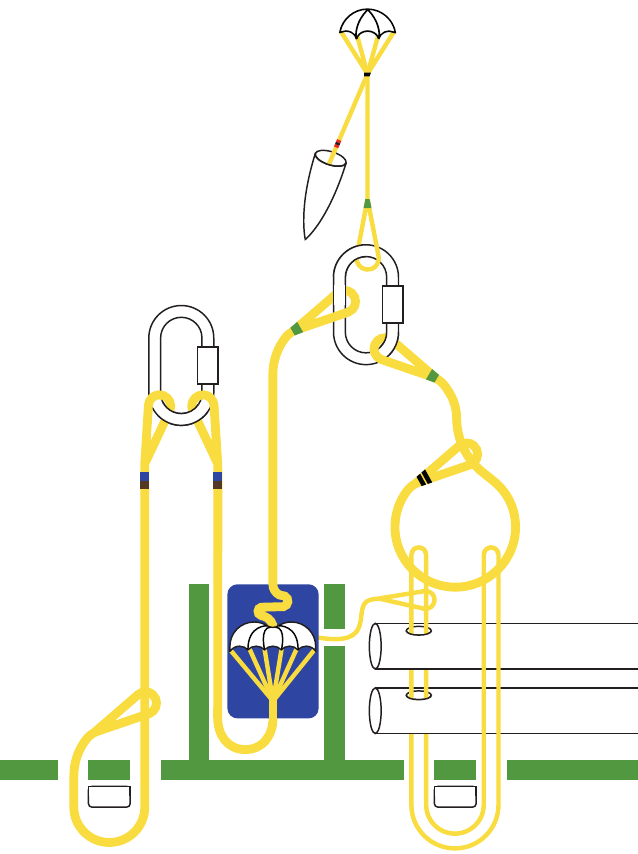
\includegraphics[width=0.7\linewidth]{recovery.png}
        \caption{Recovery line setup}
        \label{fig:chutes}
    \end{figure}
    \item Using loctite, screw upper clampband screws into upper clampband coupler without threads sticking out \checkbox
    \item Push rubber bands onto screws and fix in place with cable ties \checkbox
    \item Mount clampband line to lower coupler \checkbox
    \item Mount shockbar to Recovery main tube\checkbox
    \item Slide main shock cord onto shockbar\checkbox
    \item Slide main deployment line onto shockbar (twice)\checkbox
    \item Thread main deployment line through both main\newline deployment linecutters\checkbox
    \item Mount lower clampband coupler to main tube \checkbox
    \item Slide both drogue deployment linecutter through main tube\checkbox
    \item Mount RCU to RCU cover\checkbox
    \item Mount RCU to main tube (cables connected)\checkbox
    \item Tape antenna to main tube\checkbox
    \item Ensure shock absorber is intact. No more than the first stitched fold shall be loose.\checkbox
    \item Fold main shock cord\checkbox
    \item Thread deployment bag onto deployment bag line\checkbox
    \item Fold main chute like in this video:\newline www.youtube.com/watch?v=g$\_$v6V4a9-PA\checkbox
    \item Insert main chute into deployment bag\checkbox
    \item Connect main shock cord to main chute (blue-brown)\checkbox
    \item Secure shackle with masking tape \checkbox
    \item Insert main shock cords into deployment bag\checkbox
    \item Close deployment bag\checkbox
    \item Insert deployment bag into main tube\checkbox
    \item Thread deployment bag holdback line through main tube\checkbox
    \item Connect line 2, drogue line and deployment bag line according to\newline figure \ref{fig:chutes} \checkbox
    \item Connect line 2 and deployment bag line to drogue line (green) \checkbox
    \item Secure shackle with masking tape \checkbox
    \item Connect nosecone line to drogue chute (black) \checkbox
    \item Wrap drogue shock lines around drogue chute, add two additional turns of the drogue line\checkbox
    \item Fold remaining drogue line and nose cone line individualy in a figure eight pattern \checkbox
    \item Lay drogue chute and folded lines on top off main chute\checkbox
    \item Place drogue tube on top off main tube and make sure TRS charging connector is connected\checkbox
    \item Temporarily tape together with masking tape (mark tape as RBF)\checkbox
    \item Connect clampband to clampband line \checkbox
    \item Mount payload bay to recovery section \checkbox
    \item Connect RCU to PMU (CAN/Power) \checkbox
    \item Mount main battery with zip ties \checkbox
    \item Mount backup battery with zip ties \checkbox
    \item Insert temporary RBF pin into PMU\checkbox
    \item Mount PMU \checkbox
    \item Connect cameras to PMU \checkbox
    \item Connect payload cable to PMU \checkbox
    \item Zip tie cables \checkbox

    \starttask{Non-energetic Rocket Assembly}{\hphantom{a}}
    \item \label{rocket_non_energetic_start} Check if cable management is done properly and fix if necessary\checkbox
    \item Make photos of internals for Launch Readiness Review\checkbox
    \item Mount airframe-fincan coupler to propulsion system (4 M4x10 screws)\checkbox
    \item Rotate propulsion system until connectors are on top \checkbox
    \item Ensure upper rail button T-nut is mounted to propulsion system \checkbox
    \item Slot propulsion system into body tube \checkbox
    \item Verify alignment of ox pressurant fill and vent to the respective openings in the body tube \checkbox
    \item Screw body tube to thrust structure (4 M4x10 screws)\checkbox
    \item Screw body tube to airframe-fincan coupler (4 M4x8 screws) \checkbox
    \item Rotate fuel tank assembly to correct orientation (threaded inserts aligned with holes in body tube) \checkbox
    \item Screw fuel tank assembly in place (8 M4x8 screws) \checkbox
    \item Mount upper rail button to T-nut using threadlocker\checkbox
    \item Align fuel pressurant fill with opening in body tube \checkbox
    \item Verify temporary RBF is inserted\checkbox
    \item Connect linecutters to Altimax \checkbox
    \item Verify batteries connected properly \checkbox
    \item Verify Altimax connected properly \checkbox
    \item Verify RCU connected properly \checkbox
    \item Verify SD-cards in cameras \checkbox
    \item Verify payload inserted and connected properly \checkbox
    \item Verify if clampband screws are tight \checkbox
    \item Remove runcam covers \checkbox
    \item Connect propulsion cables to recovery section \checkbox
    \item Connect umbilical cables to recovery section \checkbox
    \item Slot recovery system into body tube and fix with 8 screws\checkbox
    \item Verify that the cameras and RBF pin align with the holes\newline in the airframe.\checkbox
    \item Cover rocket with opaque cover\checkbox
    \item Swap temporary RBF pin with final RBF pin\checkbox
    \item \label{rocket_non_energetic_end} Report non-energetic rocket assembly completed to Mission Lead.\checkbox
    
    \starttask{Energetic Rocket Assembly}{\hphantom{a}}
    \item \label{rocket_energetic_start} Prepare tools for assembly \checkbox
    \begin{enumerate}
        \item Ibus size 2.5 \checkbox
        \item Torx size 6 \checkbox
        \item Torx size 8 \checkbox
        \item Torx size 20 \checkbox
        \item Face shields \checkbox
    \end{enumerate}
    \item Remove nosecone from upper clampband\checkbox
    \item Put upper clampband onto lower clampband (ensure clampband line is not pinched) \checkbox
    \item Prepare drogue deployment line \checkbox  
    \item Thread drogue deployment line through drogue deployment linecutter \checkbox
    \item Open clampband tensioner \checkbox
    \item Thread drogue deployment line through both clampband halves and knot together (as tight as possible)\checkbox
    \item Thread clampband line inbetween the couplers \checkbox
    \item Put on face shields \checkbox
    \item Temporarely affix clampband to coupler with zip tie \checkbox
    \item Connect clampband halves with tensioner (T6) \checkbox
    \item Ensure clampband halves are connectet securely \checkbox
    \item Remove zip tie \checkbox
    \item Tighten clampband (H2.5) \checkbox
    \item \label{rocket_energetic_end} Mount RBF zip tie around clampband \checkbox
    
    \item Report energetic rocket assembly complete to Mission Lead.\checkbox
    
    \starttask{Final Rocket Assembly}{\hphantom{a}}
    \item \label{rocket_final_start} Connect TRS battery to charger \checkbox
    \item Connect TRS battery to TRS \checkbox
    \item Secure TRS battery to TRS with masking tape \checkbox
    \item Install TRS in TRS tube (T20) \checkbox
    \item Tension slingshot \checkbox
    \item Mount slingshot retainer (T8) \checkbox
    \item Remove RBF tape \checkbox
    \item Mount nosecone onto upper clampband \checkbox
    \item Secure nosecone (8 screws, H2.5) \checkbox
    \item Install RBF zip tie on clampband \checkbox
    \item Connect nosecone (including upper clampband coupler) to nosecone line (red-black)\checkbox
    
    \starttask{Igniter Installation}{\hphantom{a}}
    \item Securely screw in Igniters.\checkbox
    \item Connect igniters to igniter cables.\checkbox
    \item Properly cable manage igniter cables.\checkbox
    
    \item \label{rocket_final_end} Report Rocket Final Assembly comlete to Mission Lead\checkbox

\label{end_section_rocket}
\end{enumerate}
 \cleardoublepage
\newpage
\setcounter{page}{1}
\lhead{Pad}
\lfoot{\thepage / \pageref{end_section_pressurant}}
\section*{Pad}
\begin{tcolorbox}
\color{black}

\textbf{Important Note:}\\
Tasks for Mission Control are \underline{underlined}. Mission Control needs to be told every underlined instruction.\\
Ensuring that tasks on your checklist are done is \textbf{your} responsibility.\\
Always request acknowledgement from Mission Control and verify yourself if possible.
\end{tcolorbox}
\begin{tcolorbox}
\color{black}

\textbf{Legend:}\\
CAN \underlined Controller Area Network; Data bus (orange cable)\\
ECU \underlined Engine Control Unit\\
ECUI \underlined Engine Control User Interface\\
GSE \underlined Ground Support Equipment\\
iperf \underlined Network testing tool\\
LCO \underlined Launch Control Officer\\
LRR \underlined Launch Readiness Review\\
MC \underlined Mission Control\\
PMU \underlined Power Management Unit\\
PoE \underlined Power over Ethernet\\
%PTFE seal \underlined Teflon sealing tape\\
RBF \underlined Remove Before Flight\\
RCU \underlined Radio Control Unit\\
TRS \underlined Total Recovery System (Eggtimer)\\
T<number> \underlined Torx driver of specified size\\\\

Requests \underlined Always wait for acknowledgement\\
Instruct \underlined Acknowledgment comes later\\
Check \underlined Only assessment, no corrective actions\\
Verify \underlined Corrective action included
\end{tcolorbox}

IF A CHECK FAILS AND NO OTHER MEASURE IS SPECIFIED OR THE SPECIFIED MEASURE FAILS TOO, INFORM LEAD AND AWAIT FURTHER INSTRUCTIONS

\begin{enumerate}[label=P\arabic*.]

    \item READ THE WHOLE CHECKLIST BEFORE STARTING \checkbox

    \starttask{Required tools, materials and personnel}{\hphantom{a}}
    \item \label{pad_personnel} Personnel
        \begin{enumerate}[label*=\arabic*.]
            \item Pad 1: Daniel Frank
            \item Pad 2: Michael Pohn
            \item Pad 3: Florian Dellekart
            \item Pad 4: Bernhard Hansemann
            \item Documentation: Liana Gferer
        \end{enumerate}
    \item \label{pad_tools} Tools \checkbox
        \begin{enumerate}[label*=\arabic*.]
            \item Hammer\leftcheckbox
            \item T10 Key\leftcheckbox
            \item T30 Key\leftcheckbox
            \item Allen Key \SI{2.5}{\milli\meter}\leftcheckbox
            \item Ethanol Fueling Syringe\leftcheckbox
            \item Tweezers\leftcheckbox
            \item Fire extinguisher\leftcheckbox
        \end{enumerate}
    \item \label{pad_materials} Materials \checkbox
        \begin{enumerate}[label*=\arabic*.]
            \item Red pendant\leftcheckbox
            \item Ice or dry ice (min. \SI{3}{\kilo\gram})
            \item Oxidizer bottle mounting plate\leftcheckbox
            \item Heat exchanger tube\leftcheckbox
            \item Oxidizer Bottle\leftcheckbox
            \item Ethanol Bottles (\SI{2}{\liter})\leftcheckbox
            \item Flame Diverter\leftcheckbox
            \item Rocket (without fincan)\leftcheckbox
            \item Fincan\leftcheckbox
            \item 8x black M4 screws(4x8 mm, 4x10 mm) for fincan \leftcheckbox
            \item RBF umbilical locking device \leftcheckbox
            \item TRS-box (ALWAYS stays with rocket) \leftcheckbox
        \end{enumerate} 
    
    \starttask{On-day pad prep}{\hphantom{a}}
    \item \label{pad_on_day_start} If not already at correct position, place trailer at final launch site.\checkbox
    \item Recheck position and angles of launch rail and realign if necessary.\checkbox
    \item Voice radio check with MC. \checkbox
    \item Open server rack and remove cover from bottom air intake.\checkbox
    \item Remove masking tape from cable outlet at the back.\checkbox
    \item Connect server rack power distributor to power.\checkbox
    \item Set up pad cams if not already done. \checkbox
    \item Verify that all Ethernet and power cables are connected correctly.\checkbox
    \item Start server if not already starting automatically.\checkbox
    \item Start heating hot water reservoir.\checkbox
    \item Start cooling cold water reservoir, refill ice periodically until \ref{vacate_pad}.\checkbox
    \item Place oxidizer bottle next to trailer \checkbox
    \item Install mounting plate on oxidizer bottle \checkbox
    \item Install Ox bottle on tanking cart \checkbox
    \item Install heat exchanger on oxidizer bottle \checkbox
    \item Connect water hoses to heat exchanger\checkbox
    \item Install Pressurant bottle\checkbox
    \item Install flame diverter\checkbox
    \item Report on-day pad preparation complete to Mission Lead\checkbox
    
    \starttask{On-day electronics check}{\hphantom{a}}
    \item \label{pad_on_day_elec_start} Wait for MC to start aligning directed radio link.\checkbox
    \item \underline{MC: check functionality of following individual sensors,}\newline\underline{no software errors}
      \begin{enumerate}[label*=\arabic*.]
            \item Hot water temperature \leftcheckbox
            \item Cold water temperature \leftcheckbox
            \item Mantle water temperature \leftcheckbox
            \item Pressurant pressure \leftcheckbox
            \item Ox pressure \leftcheckbox
      \end{enumerate}
  \item \underline{MC:
    check functionality of actuators (verify movement and calibration)}
    \newline\underline{Software reports no errors and visual inspection of actuator movement}
      \begin{enumerate}[label*=\arabic*.]
            \item Ox tanking valve \leftcheckbox
            \item Ox vent valve \leftcheckbox
            \item Pressurant tanking valve \leftcheckbox
            \item Pressurant vent valve \leftcheckbox
            \item Umbilical retract \leftcheckbox
            \item Clean water pump intake filters \leftcheckbox
            \item Hot water pump \leftcheckbox
            \item Cold water pump \leftcheckbox
            \item Holddown \leftcheckbox
      \end{enumerate}
    
    \item Report On-Day electronics check complete to Mission Lead.\checkbox
    \item \label{pad_on_day_elec_end} Vacate area.\checkbox
    
    \starttask{Rocket mounting}{\hphantom{a}}
    \item \label{pad_rocket_mounting_start} Pad 1 \& 2 get rocket, fincan and TRS-box to pad.\checkbox
    \item Remove sliding block from launch rail.\checkbox
    \item Verify holddown open, if not request MC to open it.\checkbox
    \item Slide rocket (without fincan) onto rail (from bottom).\checkbox
    \item Secure rocket with sliding block underneath lower rail button.\checkbox
    \item Secure holddown above lower rail button.\checkbox
    \item Verify holddown is closed and locked.\checkbox
    \item Swivel strongback into position \checkbox
    \item Attach RBF umbilical locking device \checkbox
    \item Remove cover from pressurant loading ports.\checkbox
    \item Connect Ox pressurant umbilical.\checkbox
    \item Connect Fuel pressurant umbilical.\checkbox
    \item Verify pressurant umbilicals' mechanical connection (pull umbilical), reconnect if loose\checkbox
    \item Connect Electrical umbilical and secure with masking tape.\checkbox
    \item \underline{Request active charging.}\checkbox
    \item Pull RBF Pin halfway\checkbox
    \item Cover rocket in space blanket\checkbox
    \item \label{pad_rocket_mounting_end} Report rocket mounting completed to Mission Lead\checkbox
    
    \starttask{Fueling}{\hphantom{a}}
    \item \label{pad_fueling_start} Wait for fueling request from Lead.\checkbox
    \item Verify fuel main valve is closed.\checkbox
    \item Fill fueling syringe with \SI{950}{\milli\liter} ethanol\checkbox
    \item Fuel \SI{900}{\milli\liter} \checkbox
    \item Clean up spills\checkbox
    \item Mount fincan to rocket\checkbox
    \item Secure fincan with 8 screws\checkbox
    \item Remove cover from oxidizer loading port\checkbox
    \item Connect Ox umbilical\checkbox
    \item Verify Ox umbilical mechanical connection (pull umbilical), reconnect if loose\checkbox
    \item \label{pad_fueling_end} Report that fueling is completed to Mission Lead.\checkbox

    \starttask{Final Preps}{\hphantom{a}}
    \item \label{pad_final_preps_start} Wait for Mission Lead to request Final Preps\checkbox
    \item Unfold emergency umbilical release line and extend \newline line away from pad \checkbox
    \item Clean intake filters for water pumps \checkbox
    \item Put on safety glasses, gloves, hearing protection and long sleeved shirt and trousers.\checkbox
    \item Verify holddown closed\checkbox
    \item Start pad cams\checkbox
    \item Request Pressurization clearance from EuRoC LCO\checkbox
    \item Raise red pendant\checkbox
    \item \label{open_ox} Open Ox bottle\checkbox
    \item Check for leaks (feel for air current on connections), if found inform Mission Lead, close bottle, retighten connection and goto \ref{open_ox}\checkbox
    \item \label{open_press} Open Pressurant bottle\checkbox
    \item Check for leaks (feel for air current on connections), if found inform MC, close bottle, retighten connection and goto \ref{open_press}\checkbox
    \item Read out pressurant bottle pressure and forward to Mission Lead.\checkbox
    \item Start flight on TRS\checkbox
    \item Remove RBF zip tie \checkbox
    \item Remove RBF umbilical locking device \checkbox
    \item Pull RBF pin\checkbox
    \item Report Final preps complete to Mission Lead.\checkbox
    \item \label{vacate_pad} Vacate pad\checkbox
    
    \starttask{GSE Safing}{\hphantom{a}}
    \item \label{pad_gse_safing_start} Verify no heat sources except heating element\checkbox
    \item Close Ox bottle\checkbox
    \item Close Pressurant bottle.\checkbox
    \item Unplug heating element.\checkbox
    \item Verify heating cycle is deactivated.\checkbox
    \item \label{pad_gse_safing_end} Vacate area.\checkbox
    \item Report GSE Safing done to Mission Lead.\checkbox

    
\label{end_section_pressurant}
\end{enumerate}
 \cleardoublepage
\newpage
\setcounter{page}{1}
\lhead{MC}
\lfoot{\thepage / \pageref{end_section_lead}}
\section*{Mission Control}
\begin{tcolorbox}
\color{black}

\textbf{Legend:}\\
CAN \underlined Controller Area Network; Data bus (orange cable)\\
ECU \underlined Engine Control Unit\\
ECUI \underlined Engine Control User Interface\\
GSE \underlined Ground Support Equipment\\
iperf \underlined Network testing tool\\
LCO \underlined Launch Control Officer\\
LRR \underlined Launch Readiness Review\\
MC \underlined Mission Control\\
PMU \underlined Power Management Unit\\
PoE \underlined Power over Ethernet\\
%PTFE seal \underlined Teflon sealing tape\\
RBF \underlined Remove Before Flight\\
RCU \underlined Radio Control Unit\\
TRS \underlined Total Recovery System (Eggtimer)\\
T<number> \underlined Torx driver of specified size\\\\

Requests \underlined Always wait for acknowledgement\\
Instruct \underlined Acknowledgment comes later\\
Check \underlined Only assessment, no corrective actions\\
Verify \underlined Corrective action included
\end{tcolorbox}

\begin{enumerate}[label=P\arabic*.]
    \item READ THE WHOLE CHECKLIST BEFORE STARTING \checkbox
    
    \starttask{Required tools, materials and personnel}{\hphantom{a}}
    \item \label{mc_personnel} Personnel
        \begin{enumerate}[label*=\arabic*.]
            \item Mission Control: Markus Pinter\leftcheckbox
        \end{enumerate} 
    \item \label{mc_materials} Materials
        \begin{enumerate}[label*=\arabic*.]
            \item 2x External Screen + Power Adapter \& Cable\leftcheckbox
            \item 16-port Switch + Power Adapter\leftcheckbox
            \item Ethernet Cables (1x\SI{10}{\meter}, 2x short (1-\SI{2}{\meter}), 1x\SI{20}{\meter})\leftcheckbox
            \item Cable Reel\leftcheckbox
            \item 6-port power distributor\leftcheckbox
            \item Mission Control Laptop + Charger + Mouse\leftcheckbox
            \item Directed Radio Link dish\leftcheckbox
        \end{enumerate} 
        
    \starttask{Mission Control Prep}{\hphantom{a}}
    \item \label{mc_prep_start} Get power with cable reel and power distributor\checkbox
    \item Set up external screens, laptop and switch.\checkbox
    \item Connect the radio link and laptop to switch.\checkbox
    \item Request On-Day electronics check from Pad crew.\checkbox
    \item Verify bandwidth with iperf. Min: 10Mb/s, Target: >50Mb/s, if insufficient, request realignment.\leftcheckbox
    \item Start software infrastructure.\checkbox
    \item Confirm network with sensor readings and actuator movements.\checkbox
    \item \label{mc_prep_end} Check Holddown Servo start and end point.\checkbox
\end{enumerate}
 \cleardoublepage
\newpage
\setcounter{page}{1}
\lhead{Igniter}
\lfoot{\thepage / \pageref{end_section_igniter}}
\section*{Igniter}
%\begin{tcolorbox}
\color{black}

\textbf{Important Note:}\\
Tasks for Mission Control are \underline{underlined}. Mission Control needs to be told every underlined instruction.\\
Ensuring that tasks on your checklist are done is \textbf{your} responsibility.\\
Always request acknowledgement from Mission Control and verify yourself if possible.
\end{tcolorbox}
\begin{tcolorbox}
\color{black}

\textbf{Legend:}\\
CAN \underlined Controller Area Network; Data bus (orange cable)\\
ECU \underlined Engine Control Unit\\
ECUI \underlined Engine Control User Interface\\
GSE \underlined Ground Support Equipment\\
iperf \underlined Network testing tool\\
LCO \underlined Launch Control Officer\\
LRR \underlined Launch Readiness Review\\
MC \underlined Mission Control\\
PMU \underlined Power Management Unit\\
PoE \underlined Power over Ethernet\\
%PTFE seal \underlined Teflon sealing tape\\
RBF \underlined Remove Before Flight\\
RCU \underlined Radio Control Unit\\
TRS \underlined Total Recovery System (Eggtimer)\\
T<number> \underlined Torx driver of specified size\\\\

Requests \underlined Always wait for acknowledgement\\
Instruct \underlined Acknowledgment comes later\\
Check \underlined Only assessment, no corrective actions\\
Verify \underlined Corrective action included
\end{tcolorbox}

\begin{enumerate}[label=R\arabic*.]

    \item READ THE WHOLE CHECKLIST BEFORE STARTING \checkbox
    
    \starttask{Required tools, materials and personnel}{\hphantom{a}}
    \item \label{igniter_personnel} Personnel
        \begin{enumerate}[label*=\arabic*.]
            \item Igniter 1: Liana Gfrerer
            \item Igniter 2: Marianne Röchling
        \end{enumerate}
    \item \label{igniter_tools} Tools
        \begin{enumerate}[label*=\arabic*.]
            \item Box Cutter\leftcheckbox
            \item White Permanent Marker\leftcheckbox
            \item Thin Stick\leftcheckbox
            \item Scale\leftcheckbox
            \item Safety Glasses\leftcheckbox
            \item Hand Gloves\leftcheckbox
            \item Small Spoon\leftcheckbox
            \item Hot Plate\leftcheckbox
        \end{enumerate}
    \item \label{igniter_materials} Materials
        \begin{enumerate}[label*=\arabic*.]
            \item 6x E-Matches \leftcheckbox
            \item 6x 3D-printed Cartridges \leftcheckbox
            \item 6x Teflon Seal Discs\leftcheckbox
            \item KNO3\leftcheckbox
            \item Sugar\leftcheckbox
            \item Mg\leftcheckbox
        \end{enumerate} 
    
    \starttask{Prepare Igniters}{\hphantom{a}}
%   \item Print cartridges (min. 5) \leftcheckbox
    \item \label{rocket_prep_igniters_start} Wait for request igniter preparation from Mission Lead\checkbox
    \item Request igniter preparation clearance from EuRoC staff.\checkbox
    \item Insert e-matches into cartridges \checkbox
    \item strip insulation, cut e-match wires to length, bend wires \checkbox
    \item Label each igniter with a number \checkbox
    \item Weigh each cartridge with e-match, note masses \checkbox
    \item Mix powdered ingredients \checkbox
    \begin{itemize}
        \item \SI{3.0}{\gram} KNO3
        \item \SI{2.0}{\gram} Sugar
        \item \SI{1.5}{\gram} Mg
    \end{itemize}
    \item Cook mixture at \SI{230}{\celsius} until sticky/mushy, stirring constantly \checkbox
    \begin{itemize}
        \item Wear safety glasses, mixture could ignite.
        \item Wear hand gloves
        \item If mixture starts smoking, turn down the heat, else it will ignite.
    \end{itemize}
    \item Fill cartridges with mixture \checkbox
    \begin{itemize}
        \item Avoid leaving voids, use thin stick.
        \item Make contact with but don't fully cover e-matches
    \end{itemize}
    \item Let igniters cool down \checkbox
    \item Weigh each igniter, note masses \checkbox
    \item Photograph each igniter with the top and number visible \checkbox
    \item Request igniter test clearance from EuRoC staff\checkbox
    \item \label{rocket_prep_igniters_end} Test batch, document on video \checkbox
    \begin{itemize}
        \item Burn excess mixture
        \item Test one igniter (note number)
    \end{itemize}

\label{end_section_igniter}
\end{enumerate}
 \cleardoublepage
\newpage
\setcounter{page}{1}
\lhead{Streaming}
\lfoot{\thepage / \pageref{end_section_streaming}}
\section*{Streaming}
\begin{tcolorbox}
\color{black}

\textbf{Legend:}\\
CAN \underlined Controller Area Network; Data bus (orange cable)\\
ECU \underlined Engine Control Unit\\
ECUI \underlined Engine Control User Interface\\
GSE \underlined Ground Support Equipment\\
iperf \underlined Network testing tool\\
LCO \underlined Launch Control Officer\\
LRR \underlined Launch Readiness Review\\
MC \underlined Mission Control\\
PMU \underlined Power Management Unit\\
PoE \underlined Power over Ethernet\\
%PTFE seal \underlined Teflon sealing tape\\
RBF \underlined Remove Before Flight\\
RCU \underlined Radio Control Unit\\
TRS \underlined Total Recovery System (Eggtimer)\\
T<number> \underlined Torx driver of specified size\\\\

Requests \underlined Always wait for acknowledgement\\
Instruct \underlined Acknowledgment comes later\\
Check \underlined Only assessment, no corrective actions\\
Verify \underlined Corrective action included
\end{tcolorbox}

\begin{enumerate}[label=S\arabic*.]
    \item READ THE WHOLE CHECKLIST \checkbox
    
    \starttask{Required tools, materials and personnel}{\hphantom{a}}
    \item Streamer: Luis Büchi
    \item Stream Support: Paula-Maria Handle
    \item Streaming Laptop\checkbox
    \item Power extension cord\checkbox
    \item Webcam and Microphone\checkbox
    \item 1x \SI{10}{\meter} Ethernet cable\checkbox
    
    \starttask{Streaming}{\hphantom{a}}
    \item Take place as far away as possible from MC while still being able to connect to power and network.\checkbox
    \item Lay extension cord \& networking cable to laptop and connect.\checkbox
    \item Check network camera streams working and prepare VLC media player for direct recording.\checkbox
    \item Start OBS and set up stream info.\checkbox
    \item Test Network Camera Recording as bandwidth check.\checkbox
    \item Wait for proper time to start streaming.\checkbox
    \item On OxFill Go/NoGo, start Network Camera Recording.\checkbox
    
    
    
\label{end_section_streaming}
\end{enumerate}
 \cleardoublepage
}
\end{document}